\setcounter{chapter}{4}
\chapter{Modelling}
\label{chap:modelling}
% \minitoc
% 
% 
% \subsection{Geometry of Nerve Fibers}
% The first requirement for implementing nerve fiber models is a geometric description of the structure.
% Since the models should contain an extremely large number of nerve fibers, an optimization-friendly approach is required.
% also the determination of collisions is required.
% For this purpose simple geometries like spheres or cubes are suitable.
% %
% For this purpose, it was decided to approximate nerve fibers as tubes divided into rigid segments.
% %
% %
% %
% \subsubsection{Axon}
% \subsubsection{Myelin}
% %
% \subsection{Algorithm}
% %
% \begin{figure}[!tbh]
%     \resizebox{\textwidth}{!}{
%     \inputtikz{gfx/model/tube.tikz}}
% 	\label{fig:model_tube}
% 	\caption{tube -> ZEIG STRICHZEICHNUNG}
% \end{figure}
% %
% \subsubsection{World}
% \subsubsection{Collision Detection}
% %
% \subsection{Manipulations}
% \subsubsection{Repulsive Force}
% \subsubsection{Curvature}
% \subsubsection{Segment redivision}
% %
% \subsubsection{Structure}

% \begin{lstfloat}[!tb]
% 	\lstinputlisting[language=Python]{code/model_solver.py}
% 	\label{alg:model_solver}
% 	\caption{Exemplary execution of fastpli.model.solver}
% \end{lstfloat}
% %
% \subsection{Limitations}
% \subsubsection{Runtime}
%
\comment{\paragraph{Ziele:} 
\begin{itemize}
    \item Aufbau VCS Pipeline
    \item Umsetzungen der einzelner Funktionen und deren Nutzen
    \item 
\end{itemize}}
% 
\section{Introduction}
\cite{Balls2009}
% 
\begin{itemize}
    \item current techniques
    \item their limitations
    \item collisions
    \item link to \cite{matuschke2019}
\end{itemize}
% 
\section{\VCS}
% 
\begin{figure}[!tbh]
    \centering
    % \resizebox{.5\textwidth}{!}{
    \def\tikzwidth{0.5\textwidth}
    \inputtikz{gfx/model/conical_capsule.tikz}
    % }
    \tikzexternaldisable
	\caption[cc and co]{\Acf{CC}: \raisebox{.25em}{\tikz \draw[black](0,0)--(0.275,0);} \ac{CC}, \raisebox{.25em}{\tikz \draw[blue, dash pattern=on 2.5pt off 2.5pt](0,0)--(0.275,0);} capsule, \raisebox{.25em}{\tikz \draw[red, dash pattern={on 2.5pt off 0.9pt on 0.42pt off 0.9pt}](0,0)--(0.275,0);} bounding box}
	\tikzexternalenable
	\label{fig:conical_capsule}
\end{figure}
% 
This Method aims to model densly \ac{WM}.
The main component inside \ac{WM} consist of an Axon and its surrounding Myeling [see \dummy].
The Myelin itself is split into several parts to allow the propagation of the action potential at the Nodes of Ranvier. \\
% 
This structure is modelled as a chain of capsules, a cylinder with hemispherical ends \cref{fig:conical_capsule}.
To allow a change of cross section or radii, the capsule ending are allowed to consist of individual radii.
The resulting shape will be referred to as a \ac{CC}.
The chain of \ac{CC} consist therefore of a list of 3d points with individual radius. \\
% 
To model flexible and curved densly packed nerve fibers, a collision free result needs to be obtained.
The representaion of nerve fibers by \ac{CC} allows a fast calculation if two \ac{CC} are colliding each other. \\
% 
However instead of building a collision free model, which is quite impossible for a \dummy structure, the strategy is to initialize a model, checking for collisions and then solving these collisions by pushing the fiber or \ac{CC} slightly apart. \\
% 
This allows a user to specify any initial configuration and reaching a collision free model, which, depending on the initial overlap, follows the initial geometry.
The disadvantage obvious is that the configuration has to change.
However since biological tissue is deformable and not "caotic" itself, it follows its natrual behavier.
%
% 
% 
\section{Collision Detection}
% 
Collision detection for a large number of objects is a very computational intense algorithm.
To reduce the computational afford, the \ac{CC} will be interpreted as a capsule object, since this alows a much simpler calculation.
The capsule has the radius $r_{\text{capsule}} = \max(r_0, r_1)$ to soroun the hole \ac{CC}.
To check if two capsules collide with each other the distance between the line segments, defined by the capsule begin and end points $p_0, p_1$, is calculated.if the distance $d$ is $d < (r_0 + r_1)$ then the two capsule objects are colliding each other. \\
% 
To calculate the smallest distance between two line segemnts, sevverel algorith,s already exists.
A fast approach was chosen\footnote{\href{https://www.john.geek.nz/2009/03/code-shortest-distance-between-any-two-line-segments/}{https://www.john.geek.nz/2009/03/code-shortest-distance-between-any-two-line-segments/}}.
%
\section{World}
For a given cuboid volume the computing grows $\mathcal{O}(V^3)$.
Furthermore each object has to be checked to each other, therefore the number of objects to be checked for a collision grows by $\mathcal{O}(n^2)$.
This explodes rather quick.
In the literature are several approuches (e.g. computer games industry).
However since the number of objects will be $\approx \num{e9}$ \dummy cant be used. \\
% 
A "tree" is a data structure consist of a collection of "nodes", which are connected to each other.
One node is conected toword the "root" with a single parent node and towords the "branches" with several "children" or "branches".
The nodes at the end of a branch are refered to as "leafs" wich contain the data.
Traversing a  evenly distributed tree is of $\mathcal{O}(\log(n))$.\\
% 
\begin{figure}[!tb]
    \centering
    \subcaptionbox{oct tree}[.3\textwidth]{
    \def\tikzheight{0.6\textwidth}
    \def\zangle{50}
\def\xangle{-0}
% 
\begin{tikzsize}{\textwidth}
\begin{tikzpicture}[scale=\tikzscale,
                    x=(\xangle:1cm), y=(90:1cm), z=(\zangle:0.5cm)]
    % % 
    % \draw (0,0,0)--(1,0,0) node[midway] {x};
    % \draw (0,0,0)--(0,1,0) node[midway] {y};
    % \draw (0,0,0)--(0,0,1) node[midway] {z};
    % 
    \begin{scope}[local bounding box=BB1]
    \draw[thick] (0,0,0)--(1,0,0){};
    \draw[thick] (0,0,0)--(0,1,0){};
    \draw[thick] (1,0,0)--(1,1,0){};
    \draw[thick] (0,1,0)--(1,1,0){};
    \draw[thick] (1,1,0)--(1,1,1){};
    \draw[thick] (1,0,0)--(1,0,1){};
    \draw[thick] (0,1,0)--(0,1,1){};
    \draw[thick] (0,1,1)--(1,1,1){};
    \draw[thick] (1,0,1)--(1,1,1){};
    \end{scope}
    % 
    \begin{scope}[yshift = -2cm, local bounding box=BB2]
    \draw[thick] (0,0,0)--(1,0,0){};
    \draw[thick] (0,0,0)--(0,1,0){};
    \draw[thick] (1,0,0)--(1,1,0){};
    \draw[thick] (0,1,0)--(1,1,0){};
    \draw[thick] (1,1,0)--(1,1,1){};
    \draw[thick] (1,0,0)--(1,0,1){};
    \draw[thick] (0,1,0)--(0,1,1){};
    \draw[thick] (0,1,1)--(1,1,1){};
    \draw[thick] (1,0,1)--(1,1,1){};
    % 
    \draw[] (1,1,0.5)--(1,0,0.5){};
    \draw[] (1,1,0.5)--(0,1,0.5){};
    \draw[] (0.5,1,0)--(0.5,0,0){};
    \draw[] (0.5,1,0)--(0.5,1,1){};
    \draw[] (0,0.5,0)--(1,0.5,0){};
    \draw[] (1,0.5,1)--(1,0.5,0){};
    \end{scope}
    % 
    \begin{scope}[yshift = -4cm, local bounding box=BB3]
    \draw[thick] (0,0,0)--(1,0,0){};
    \draw[thick] (0,0,0)--(0,1,0){};
    \draw[thick] (1,0,0)--(1,1,0){};
    \draw[thick] (0,1,0)--(1,1,0){};
    \draw[thick] (1,1,0)--(1,1,1){};
    \draw[thick] (1,0,0)--(1,0,1){};
    \draw[thick] (0,1,0)--(0,1,1){};
    \draw[thick] (0,1,1)--(1,1,1){};
    \draw[thick] (1,0,1)--(1,1,1){};
    % 
    \draw[] (1,1,0.5)--(1,0,0.5){};
    \draw[] (1,1,0.5)--(0,1,0.5){};
    \draw[] (0.5,1,0)--(0.5,0,0){};
    \draw[] (0.5,1,0)--(0.5,1,1){};
    \draw[] (0,0.5,0)--(1,0.5,0){};
    \draw[] (1,0.5,1)--(1,0.5,0){};
    % 
    \draw[very thin] (0.75,0.5,0)--(0.75,1,0){};
    \draw[very thin] (0.5,0.75,0)--(1,0.75,0){};
    \draw[very thin] (0.75,1,0)--(0.75,1,0.5){};
    \draw[very thin] (0.5,1,0.25)--(1,1,0.25){};
    \draw[very thin] (1,0.75,0)--(1,0.75,0.5){};
    \draw[very thin] (1,0.5,0.25)--(1,1,0.25){};
    \draw[very thin] (0.25,0,0)--(0.25,0.5,0){};
    \draw[very thin] (0,0.25,0)--(0.5,0.25,0){};
    \end{scope}
    % 
    \draw[->] ($(BB1.south) - (0,0.1)$) -- ($(BB2.north) + (0,0.1)$){};
    \draw[->] ($(BB2.south) - (0,0.1)$) -- ($(BB3.north) + (0,0.1)$){};
    % 
    \node[above, anchor=south, xshift=-1ex,rotate=90] at (BB1.west) {\scriptsize level=0};
    \node[above, anchor=south, xshift=-1ex,rotate=90] at (BB2.west) {\scriptsize level=1};
    \node[above, anchor=south, xshift=-1ex,rotate=90] at (BB3.west) {\scriptsize level=2};
    % 
\end{tikzpicture}
\end{tikzsize}
    }
    \subcaptionbox{collision 2d}[.65\textwidth]{
    \def\tikzheight{0.6\textwidth}
    \begin{tikzsize}{\textwidth}{\tikzheight}
\begin{tikzpicture}[scale=\tikzscale]
    % \draw (0,0) grid (10,10);
    \path (0,0) -- (10,10);
    \begin{scope}[shift={(0.75,3)},local bounding box=BB1]
        \draw (0:1cm) \foreach \x in {0,120,...,360} {-- (\x:1cm)} -- cycle {};
        \node (0,0) {obj 1};
    \end{scope}
    % 
    \begin{scope}[shift={(7,4.8)},local bounding box=BB2]
        \draw (0:1cm) \foreach \x in {0,60,...,360} {-- (\x:1cm)} -- cycle {};
        \node (0,0) {obj 2};
    \end{scope}
    % 
    \begin{scope}[shift={(5.5,8)},local bounding box=BB3]
        \draw (0:1cm) \foreach \x in {0,90,...,360} {-- (\x:1cm)} -- cycle {};
        \node (0,0) {obj 3};
    \end{scope}
    % 
    \draw[thick, red] (BB1.north west) rectangle (BB1.south east);
    \draw[thick, red] (BB2.north west) rectangle (BB2.south east);
    \draw[thick, red] (BB3.north west) rectangle (BB3.south east);
    % 
    \draw[thick] (0,0) rectangle (10,10);
    % 
    \draw[] (5,0) -- (5,10);
    \draw[] (0,5) -- (10,5);
     % 
    \draw[thin] (5,7.5) -- (10,7.5);
    \draw[thin] (7.5,5) -- (7.5,10);
    % 
    \node at (2.5, 2.5) {$(0,0)$};
    \node at (7.5, 2.5) {$(1,0)$};
    \node at (2.5, 7.5) {$(0,1)$};
    % 
    \node at (6.25, 6.25) {$(10,10)$};
    \node at (8.75, 6.25) {$(11,10)$};
    \node at (6.25, 8.75) {$(10,11)$};
    \node at (8.75, 8.75) {$(11,11)$};
\end{tikzpicture}
\end{tikzsize}
    }
	\caption{}
	\label{fig:oct_tree}
\end{figure}
% 
An octtree is a special kind of tree where each node contain 8 children.
This allows to divide a cubic volume into 8 equal cutted subcubes.
Therefore this data structure was chosen to reorder the fiber segents.
To order them, a recursive function is used.
It checks, if the number of objects is below a threshold $n < t_n$, or the subvolume cube length is below a threshold $dim < t_{dim}$.
If so, the leaf is reached and all objects are check for collision with each other.
Otherwise a 8 new subvolumes will be created and each object will be check, if it is inside upto 8 of the new created volumes.
The next branch will check only with the new includes objects. \\
% 
This allows a rather quick reduction of number of objects to be checked.
Therefore the last step with an $\mathcal{O}(n^2)$ is not that painful anymore.
To speed up the calculation, The objects itself wont be duplicated.
All objects are contained in a \textit{std::vector} of cones.
Only the indices will be transfered to the next recursive function call.
Also the objects are traversed in order, so that the maximum speed from the cpu cache can be exploited. \\
% 
The minimal subvolume size is choses to $\sqrt{3} \times \max(\text{object size})$.
Smaller then this would only replicated subvolumes with identical contained objects.
The maximum number of objects is set to \num{25} objects \footnote{found suitable by testing.}. \\
% 
The building of the tree is don in parallel.
Up to 8 threads are spawned to check for the first 8 subvolumes, which objects are contained.
The next level can again spawn upto 8 new threads (64 in total).
This compensates if a the objects are not uniformly distributed.
After the first level, each cpu thread traverses it branch.
At each leaf a list ob object is returned containing the object of the leaf.
All list are collected for the collision checking test.
This collected list is in the next step fully parallel traversed to check for collisions.
% 
\subsection{Solving a collision}
To solve a collision between two \ac{CC} objects the two points of each object will be moved.
The movement will be parallel to the smallest distance line between both objects.
To take the 3d placement into consideration, the movement is weighted with the distance of the the individual points to the intersection point with the smallest distance line (see fig \dummy).
This will result in a more controlled movement if \eg only the two endings of the fiber objects collide each other. \\
% 
The movement is saved for each object in a velocity \textit{std::vector}.
Therefore the sum of all velocities is taken into account.
The maximum speed is however limited to a value of $v_{\max} = 0.1 \times \min(object radius)$.
This prevents movement through another object.
% 
\subsection{Shape Control}
The movement of individual points can results in a "distorted" fiber model, \eg two points move very far apart from each other.
Therefore boundry conditions have to be specified.
It was decided to use the following two conditions:
% 
\subsubsection{Mean segment length}
% 
\begin{figure}[!tb]
    \subcaptionbox{}[0.5\textwidth]{
\def\tikzwidth{.5\textwidth}
\begin{tikzsize}{\tikzwidth}{\tikzheight}
\begin{tikzpicture}[scale=\tikzscale,]
% 
\draw[lightgray,rounded corners,line width=42pt] (0,0)
\foreach \i in {(2,1),(4,-1),(6,0.75),(8,-0.15)}{
-- \i} -- (10,0.42);
% 
\foreach \p [count=\i] in {(0,0),(2,1),(4,-1),(6,0.75),(8,-0.15),(10,0.42)}{
\draw[lightgray, fill] \p circle (21pt); 
\pgfmathsetmacro{\ii}{int(\i-1)}
\draw[black, fill] \p circle (2pt) node[black, yshift=-5pt, anchor=north] {$p_{\ii}$};}
% 
% 
\begin{scope}[shift={(0,-4.2)}]
\draw[lightgray,rounded corners,line width=42pt] (0,0)
\foreach \i in {(4,-1),(8,-0.15)}{
-- \i} -- (10,0.42);
% 
\foreach \p [count=\i] in {(0,0),(4,-1),(8,-0.15),(10,0.42)}{
\draw[lightgray, fill] \p circle (21pt); 
\pgfmathsetmacro{\ii}{int(\i-1)}
\draw[black, fill] \p circle (2pt) node[black, yshift=-5pt, anchor=north] {$p'_{\ii}$};}
\end{scope}
% 
\end{tikzpicture}
\end{tikzsize}  
% \resizebox{0.5\textwidth}{!}{
% \begin{tikzpicture}[]
% % 
% \path [] (-13,-9) grid (13,9);
% % 
% \begin{scope}[shift={(-7,0)}]
% \foreach \pa/\pb/\ra/\rb [count=\ii] in {
% (-1,5)/{(3,1)}/3/2,
% (3,1)/{(-3,-5)}/2/2.5
% } {
%     \def\l{c\ii}
%     % 
%     \pgfmathsetmacro{\rone}{\ra}
%     \pgfmathsetmacro{\rtwo}{\rb}
%     \pgfmathsetmacro{\out}{\rone/(\rone - \rtwo)}
%     \node[draw, circle,minimum size=2 * \rone cm,inner sep=0pt] (\l1) at \pa {};
%     \node[circle,minimum size=2 * \rtwo cm,inner sep=0pt] (\l2) at \pb {};
%     \path (\l1.center) -- node[coordinate,pos=\out] (out) {}  (\l2.center);
%     % 
%     \foreach \i in {1,2}
%     \foreach \j in {1,2}
%     \foreach \k in {out}
%     \coordinate (t\i\j\k) at (tangent cs:node=\l\i,point={(\k)},solution=\j);
%     % 
%     \foreach \i in {1,2}
%     \foreach \k in {out}
%     \draw[red] ($(t1\i\k)!-0cm!(t2\i\k)$) --  ($(t2\i\k)!-0cm!(t1\i\k)$);
%     % 
%     % last circle
%     \ifnum\ii=2
%         \node[draw,circle,minimum size=2 * \rtwo cm,inner sep=0pt] (last) at \pb {};
%     \fi
% }
% \end{scope}
% % 
% \draw[very thick, ->, >=latex, line width=5pt] (-1,0) -- (1,0);
% % 
% \begin{scope}[shift={(9,0)}]
% \foreach \pa/\pb/\ra/\rb [count=\ii] in {
% (-1,5)/{(-3,-5)}/3/2.5
% } {
%     \def\l{c\ii}
%     % 
%     \pgfmathsetmacro{\rone}{\ra}
%     \pgfmathsetmacro{\rtwo}{\rb}
%     \pgfmathsetmacro{\out}{\rone/(\rone - \rtwo)}
%     \node[draw, circle,minimum size=2 * \rone cm,inner sep=0pt] (\l1) at \pa {};
%     \node[circle,minimum size=2 * \rtwo cm,inner sep=0pt] (\l2) at \pb {};
%     \path (\l1.center) -- node[coordinate,pos=\out] (out) {}  (\l2.center);
%     % 
%     \foreach \i in {1,2}
%     \foreach \j in {1,2}
%     \foreach \k in {out}
%     \coordinate (t\i\j\k) at (tangent cs:node=\l\i,point={(\k)},solution=\j);
%     % 
%     \foreach \i in {1,2}
%     \foreach \k in {out}
%     \draw[red] ($(t1\i\k)!-0cm!(t2\i\k)$) --  ($(t2\i\k)!-0cm!(t1\i\k)$);
%     % 
%     % last circle
%     \ifnum\ii=1
%         \node[draw,circle,minimum size=2 * \rtwo cm,inner sep=0pt] (last) at \pb {};
%     \fi
% }
% \end{scope}
% \end{tikzpicture}
% }
}
% 
% \newline
%
% \centering
\subcaptionbox{}[0.5\textwidth]{
\resizebox{0.5\textwidth}{!}{
\begin{tikzpicture}[]
% 
\path [] (-13,-9) grid (13,9);
% 
\begin{scope}[shift={(-7,0)}]
\foreach \pa/\pb/\ra/\rb [count=\ii] in {
(1,5)/{(-1,-5)}/2.5/2
} {
    \def\l{c\ii}
    % 
    \pgfmathsetmacro{\rone}{\ra}
    \pgfmathsetmacro{\rtwo}{\rb}
    \pgfmathsetmacro{\out}{\rone/(\rone - \rtwo)}
    \node[draw, circle,minimum size=2 * \rone cm,inner sep=0pt] (\l1) at \pa {};
    \node[circle,minimum size=2 * \rtwo cm,inner sep=0pt] (\l2) at \pb {};
    \path (\l1.center) -- node[coordinate,pos=\out] (out) {}  (\l2.center);
    % 
    \foreach \i in {1,2}
    \foreach \j in {1,2}
    \foreach \k in {out}
    \coordinate (t\i\j\k) at (tangent cs:node=\l\i,point={(\k)},solution=\j);
    % 
    \foreach \i in {1,2}
    \foreach \k in {out}
    \draw[red] ($(t1\i\k)!-0cm!(t2\i\k)$) --  ($(t2\i\k)!-0cm!(t1\i\k)$);
    % 
    % last circle
    \ifnum\ii=1
        \node[draw,circle,minimum size=2 * \rtwo cm,inner sep=0pt] (last) at \pb {};
    \fi
}
\end{scope}
% 
\draw[very thick, ->, >=latex, line width=5pt] (-1,0) -- (1,0);
% 
\begin{scope}[shift={(7,0)}]
\foreach \pa/\pb/\ra/\rb [count=\ii] in {
(1,5)/{(0,0)}/2.5/2.25,
(0,0)/{(-1,-5)}/2.25/2
} {
    \def\l{c\ii}
    % 
    \pgfmathsetmacro{\rone}{\ra}
    \pgfmathsetmacro{\rtwo}{\rb}
    \pgfmathsetmacro{\out}{\rone/(\rone - \rtwo)}
    \node[draw, circle,minimum size=2 * \rone cm,inner sep=0pt] (\l1) at \pa {};
    \node[circle,minimum size=2 * \rtwo cm,inner sep=0pt] (\l2) at \pb {};
    \path (\l1.center) -- node[coordinate,pos=\out] (out) {}  (\l2.center);
    % 
    \foreach \i in {1,2}
    \foreach \j in {1,2}
    \foreach \k in {out}
    \coordinate (t\i\j\k) at (tangent cs:node=\l\i,point={(\k)},solution=\j);
    % 
    \foreach \i in {1,2}
    \foreach \k in {out}
    \draw[red] ($(t1\i\k)!-0cm!(t2\i\k)$) --  ($(t2\i\k)!-0cm!(t1\i\k)$);
    % 
    % last circle
    \ifnum\ii=2
        \node[draw,circle,minimum size=2 * \rtwo cm,inner sep=0pt] (last) at \pb {};
    \fi
}
\end{scope}
\end{tikzpicture}
}}
	\caption{a) merge, b) split}
	\label{fig:merge_split}
\end{figure}
% 
% 
\begin{figure}[!tb]
    \centering
    % \resizebox{\textwidth}{!}{
    \inputtikz{gfx/model/model_length.tikz}
    % }
	\caption{different fiber segment length.}
	\label{fig:model_length}
\end{figure}
% 
The Mean segment length coresponts to the distance between the two points of an object.
If the lenght of the object becomes to small/big, the points inside a fiber coresponding to the object are merged/splitted resulting in one point less / adding a new point.
The minimum/maximum distance of the object is set to $d_{\min} = \frac{2}{3} \overline{d}, d_{\max} = \frac{4}{3}\overline{d}$.
Therefore the mean allowed value of the object is $\frac{d_{\min} + d_{\max}}{2} = \overline{d}$. \\
% 
If a new point is created due to exceeding the maximum limitation, the new points position $\vv{p}_{new}$ is 
\begin{align}
\begin{split}
\vv{p}_{new} &= \frac{\vv{p}_{i} + \vv{p}_{i+1}}{2}\\
r_{new} &= \frac{r_{i} + r_{i+1}}{2}\\
\vv{v}_{new} &= \frac{\vv{v}_{i} + \vv{v}_{i+1}}{2}
\end{split}
\end{align}
with a radius of $r_{new}$ and a velocity$\vv{v}_{new}$.
% 
\subsubsection{Bending radius}
% 
The bending radius is defined as the circular radius coresponding to the circle definded by three neigborinig points $p_{i-1}, p_{i}, p_{i+1}$. 
The limit is set as a minimal radius of $r_{\min}$.
If a point $p_{i}$ in a fiber fall below this value, the three points will be moved.
$p_{i-1},p_{i+1}$ will be moved \dummy and $p_{i}$ oposit.
Therefore the curvature will be reduced.
% 
\begin{figure}[!tb]
    \centering
    \inputtikz{gfx/model/model_radius.tikz}
	\caption{different bending radii for const fiber radius.}
	\label{fig:model_radius}
\end{figure}
% 
\begin{figure}[!tb]
    \centering
    \inputtikz{gfx/model/model_circular.tikz}
	\caption{radial ....}
	\label{fig:model_circular}
\end{figure}
% 
\begin{figure}[!tb]
    \centering
    \inputtikz{gfx/model/model_circle_.tikz}
	\caption{radial ....}
	\label{fig:model_circle_}
\end{figure}
% 
\newline
Both movements are added to the velocity vector before performing the overall movement.
The algorithm performs each step sequentially (see \cref{alg:pseudocode_solver}).
\begin{lstfloat}[!tb]
\lstset{style=cpp}

\begin{lstlisting}[]
FiberCollisionSolver(objects) {
	colliding_list = {};
	do{
		// Reset Parameter
		colliding_list.clear();
		SetSpeed(objects, 0);
		
		// Building Octree
		octree = OctTree(objects);
		
		// Collision Detection
		for ( leaf : octree ){
			colliding_objs = CheckLeaf(leaf.fiber_list());
			colliding_list.insert(colliding_objs);
		}
		
		// Seperation Process
		AddSpeed(colliding_list);
		NormalizeSpeed(colliding_list);
		MoveObject(colliding_list);
		
		// Shape Control
		SegmentLength(colliding_list, target_length);
		BendingRadius(colliding_list, target_curvature);
		
	} while (!colliding_list.empty());
}
\end{lstlisting}
\caption{Pseudocode of the main algorithm: The function \texttt{FiberCollisionSolver} will loop the followings four steps, which are run in parallel, until no collision are detected anymore: 1. build an \texttt{OctTree} from all objects, 2. \texttt{Collision Detection}, 3. \texttt{Seperation Process} and 4. \texttt{Shape Control}.}
\label{alg:pseudocode_solver}
\end{lstfloat}
% 
Finaly a volume is marked as collision free, if no collision are found and all boundry conditions are fullfiled. 
The voundry conditions can be set to 0 to ignore them.
Additionally a drag value can be set, to reduce the velocity by its factor after each step.
It can help to reach a collision free volume faster, however the density will be significantly reduced.
Therefore the value is to 0 so that after each step the velocity is resetted to $\vv{0}$. 
% 
%
% 
% 
\section{Sandbox}
% 
\section{Visualization}
% 
A visualization tool was written to visualize the fiber configuration. This allows the user a direct feedback (\eg after each step) to tune the initial fiber configuration or boundry condition. It was written in \textit{OpenGL 2}.
% 
\ac{CC} are either renderd via the \textit{gluCylinder} function provided by the \textit{GLUT} library for a rough but fast visualiation. This represents the capsule representation. For a more precise and correct visualization of the \ac{CC}, a self implemented rendering was developet. The outer hull, or mesh, is created as a tube sourounding the fiber with circular orderd poinuts around a fiber point $p_i$ (see \dummy).
% 
From the mesh, vertices and normals are calculated, which are then finaly rendered. To allow a visualization of the inner axon, the myelin hull can also be transperented rendert. This however needs sorted vertices along the z axis (inside the screen). This process takes quite some time, therefore only feasible for screenshoots at this time (see fig \dummy).
% 
\begin{figure}[!tb]
    % \resizebox{\textwidth}{!}{
    \def\tikzwidth{\textwidth}
    \inputtikz{gfx/model/vis.tikz}
    % }
	\caption{mesh}
	\label{fig:vis_mesh}
\end{figure}
% 
\paragraph{Disclamer}
This is a fast written approuch. Current rendering software uses far more advanced techniques. However this rendering algorithm was written to be a light integrated tool using only the aditional \textit{OpenGL 2} and \textit{GLUT} library.\\
% 
A more advanced Tool, the \textit{FAConstructor} \cite{Reuter2019} was written by Andr'e Reuter in the context of this doctorial research. This tool uses \textit{OpenGl 3} and additional calculation on the GPU. Additionally it allows user defined interactive technique to create a 3d fiber model.
%  
% 
% 
% 
\section{Medusa}
% 
Additionally to the previous discussed Algorithm (\dummy), the \ac{MEDUSA} algorithm, was developed in a cooperation with the team Neurospin from \ac{CEA} in France \cite{Ginsburger2019}. The targed was to develop an algorithm which can build a library of \ac{WM} tissue. This library should not only contein nerve fibers, but also other cell types like olegodendrocites or astrocytes. These cell types are currently not used in \ac{3D-PLI} routin analysis however in \ac{dMRI} the cell are quite important [\dummy]. Furthermore these cells take up additional volume which results in different nerve fiber configurations.\\
% 
Since this tool aims to build a statistically library, other parameters are chosen for boundry conditions. These parameters are chosen as close as possible from the current \ac{dMRI} models:
\dummy\\
\dummy\\
% 
% Instead of choosing \ac{CC} the fibers and cells are represented as a collection of spheres. This has the advantage that the collision of spheres are more easier to be calculated:
% \begin{align}
%     d < r_i + r_j
% \end{align}
% 
On the other side more spheres  are needed to represent a fiber. There can always be a resulting overlapp which depnding on the usecase, can lead to .. results.\\
% 
Cells are also represented as a collection of spheres, filling out the sum of the spheres volume. \\
%
In this theses cells are disregarded. A full description of the construction with astrocytes and olegodendrocytes can be found in \cite{Ginsburger2019}.
% 
\subsection{Algorithm}
% 
\begin{figure}[!tb]
\centering
% \resizebox{0.75\textwidth}{!}{
\def\tikzwidth{0.75\textwidth}
\inputtikz{gfx/model/medusa/medusa_spheres.tikz}
% }
\caption{modified from \cite{Ginsburger2019}}
\label{fig:model:medusa_4}
\end{figure}
%
% \begin{figure}[!tb]
%     \centering
%     % \resizebox{0.75\textwidth}{!}{
%     \def\tikzwidth{0.75\textwidth}
%     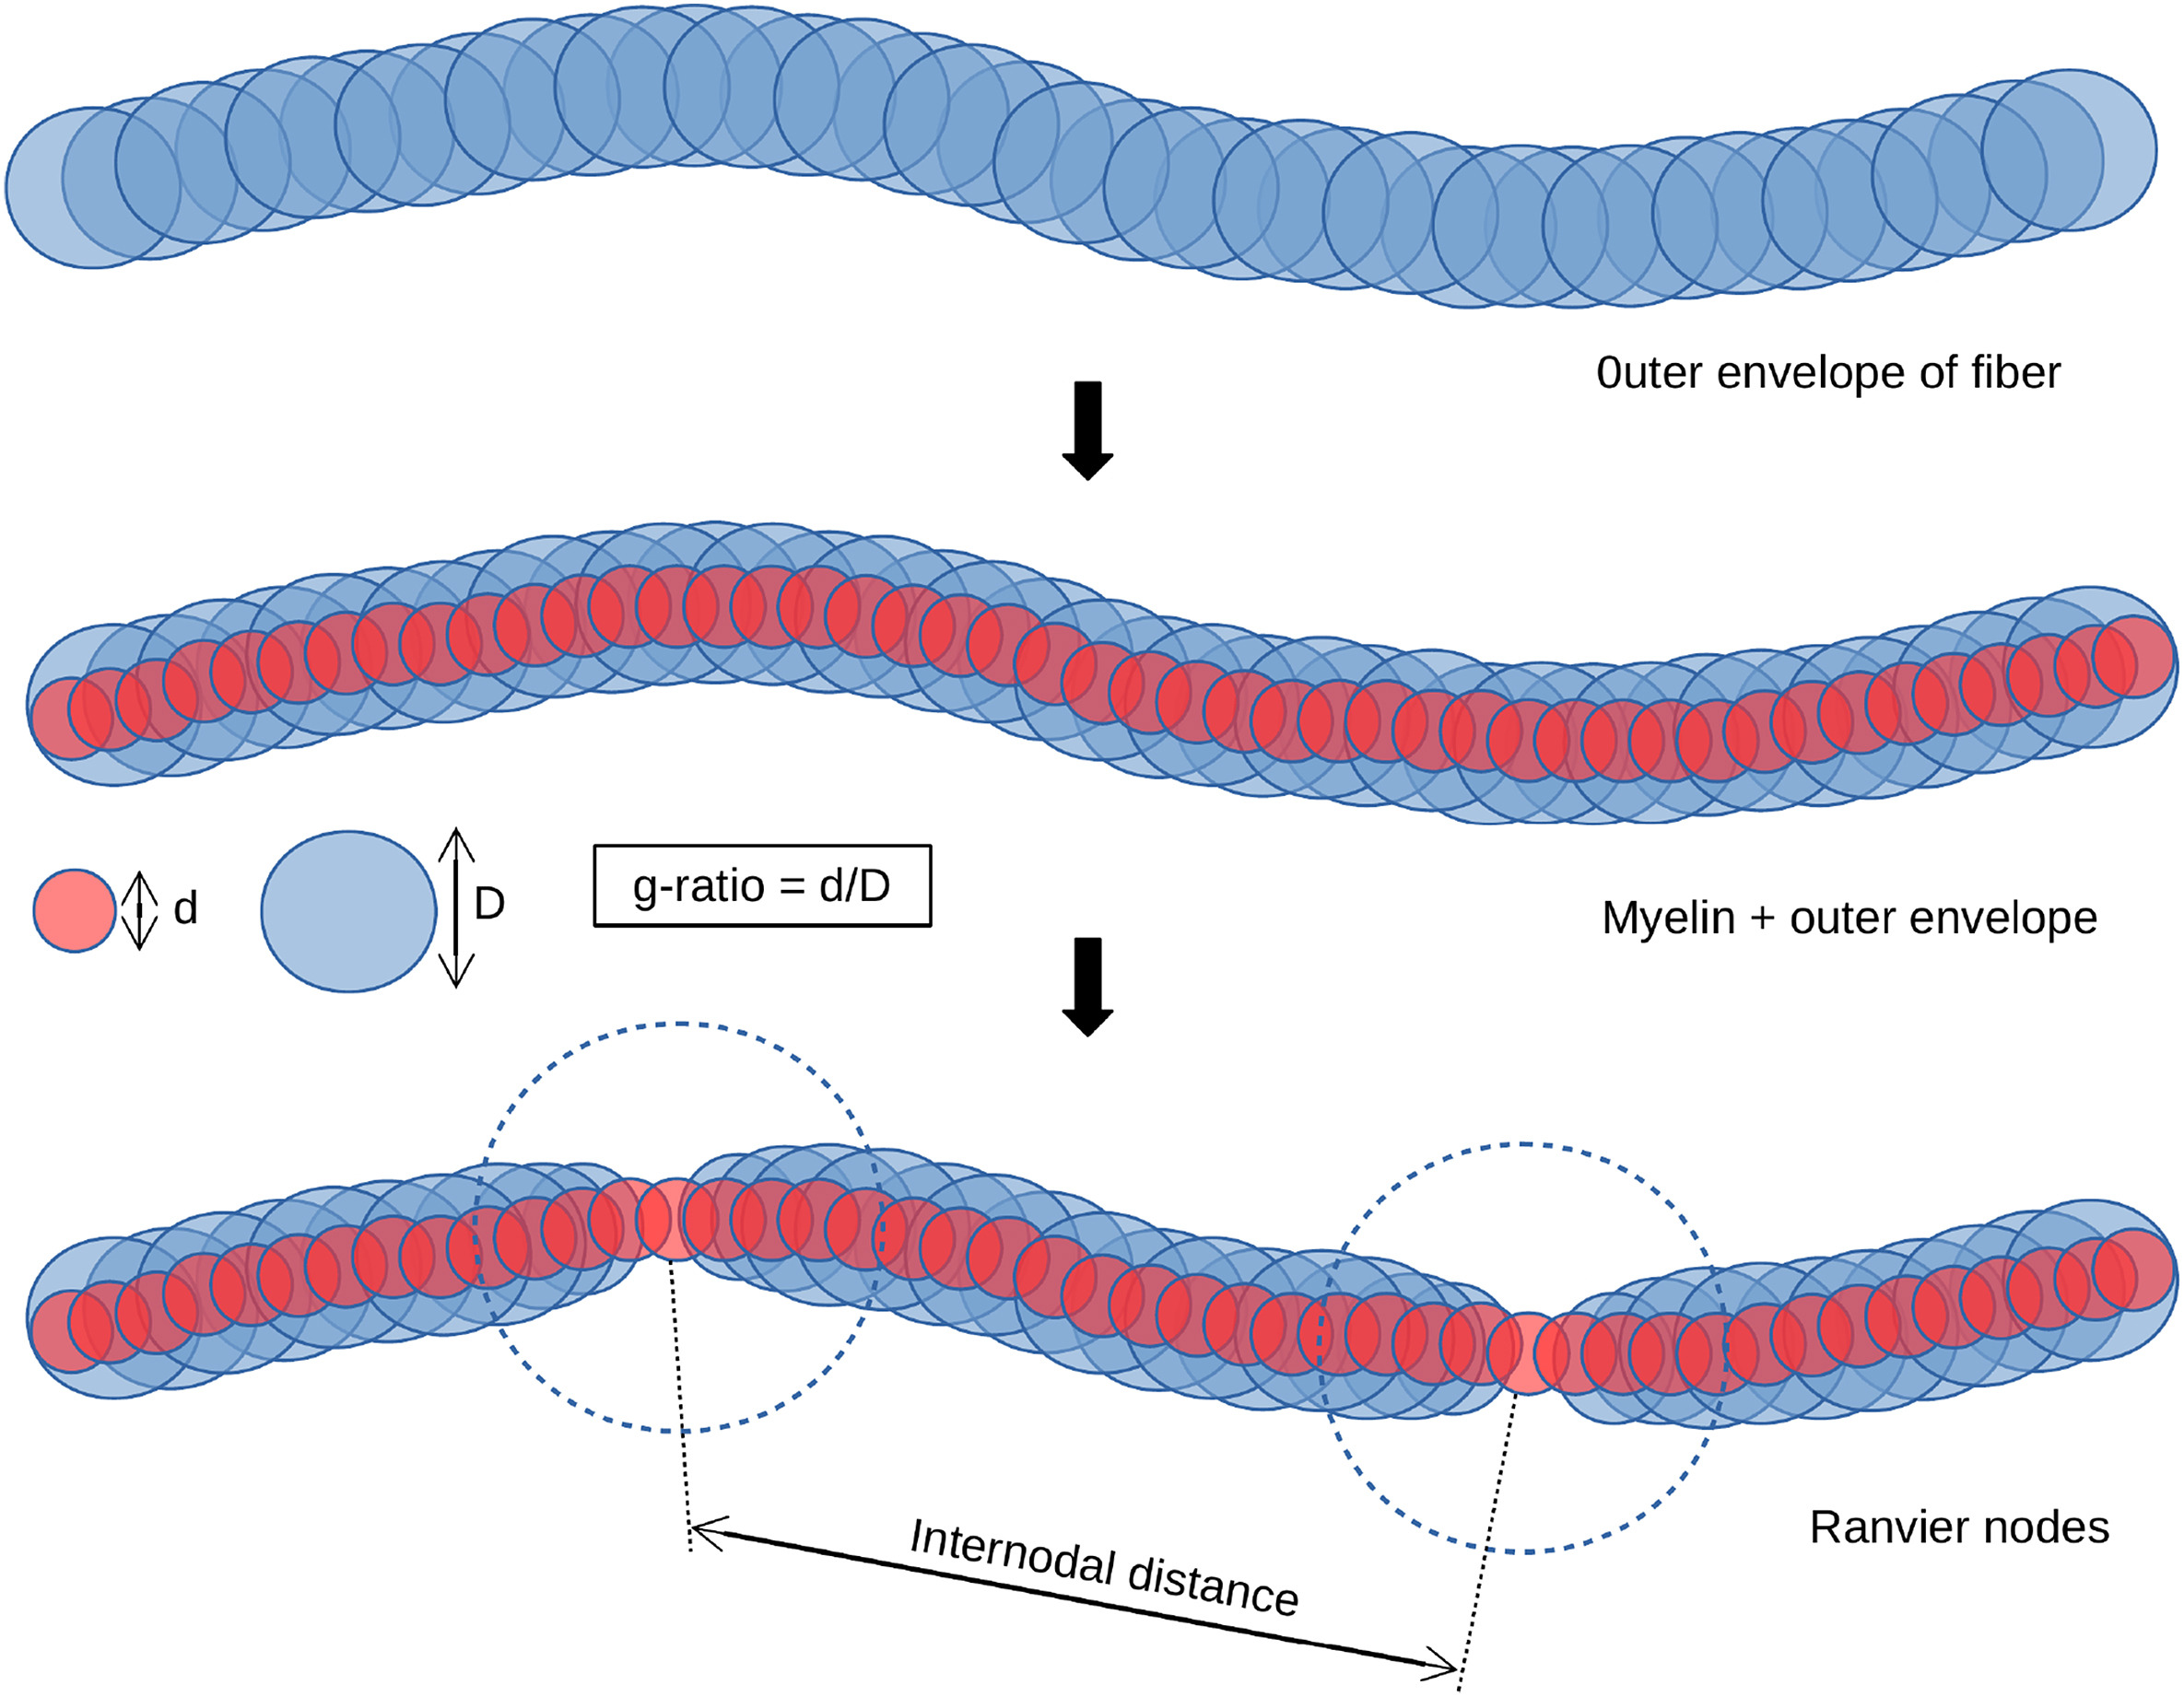
\includegraphics{gfx/model/medusa/4.jpg}
%     % }
% 	\caption{4 \cite{Ginsburger2019}}
% 	\label{fig:model:medusa_4_org}
% \end{figure}
% 
Since all objects are represented as a collection of spheres (see \cref{fig:model:medusa_4})
\begin{align}
    \mathcal{S} = \{ (x_i,y_i,z_i,r_i) : i \in \{0, 1, ..., n_\text{objects}-1\}  \} 
\end{align}
% 
, a collision is present if (VCS !!!)
% 
\begin{align}
\begin{split}
d<r_i+r_j\\
d = \abs{\vv{p}_i - \vv{p}_j}
\end{split}
\end{align}
% 
However since neighboring spheres in one fiber are colliding for a densly filled fiber, they have to be excluded if
\begin{align}
\begin{split}
d(i,j) &\leq  r_i + r_j\\
d(i,j) &= 
\begin{cases}
\sum_{n=i}^{j-1} \abs{\vv{p}_n - \vv{p}_{n+1}},& \text{if } j-i \geq 1\\
0 & \text{otherwise}
\end{cases}
\end{split}
\end{align}
% 
Spheres inside cell bodys are not checked for collision, since their volume aproximate? the volume of the cell.\\
% 
The calculation of collisions is done via the GPU architecture. For this a first implementation was written with the \textit{AxisAligedSortedSearch} \cite{Karras2012}. It sorteds the spheres along one axis, \eg x-axis, and search for each sphere the fist and last possible collision on this axis:
\begin{align}
\begin{split}
\mathcal{C}_i = \{ s \in \mathcal{S} \mid \abs{s_i.x - s_j.x} < r_i+r_j \}
\end{split}
\end{align}
% 
\begin{lstfloat}[!tb]
	\lstinputlisting[style=cpp]{code/medusa.cu}
	\caption{Pseudocode of \acs{MEDUSA} collision checking.}
	\label{alg:medusa_collision}
\end{lstfloat}
% 
The above described algorithm is currently used for volumes $\approx \SI{200}{\micro\meter}$. For this volume size the algorithm is for the current use fast enough. However, more advaned algorithm exist wich can be applied here (\eg \textit{BoundindBoxHierarchy} \cite{Karras2012}).
% 
\subsection{Results}
% 
\begin{figure}[!tb]
    \centering
    \resizebox{0.95\textwidth}{!}{
    \includegraphics{gfx/model/medusa/8.jpg}}
	\caption{8 \cite{Ginsburger2019}}
	\label{fig:medusa_8}
\end{figure}
% 
\begin{figure}[!tb]
    \centering
    \resizebox{0.95\textwidth}{!}{
    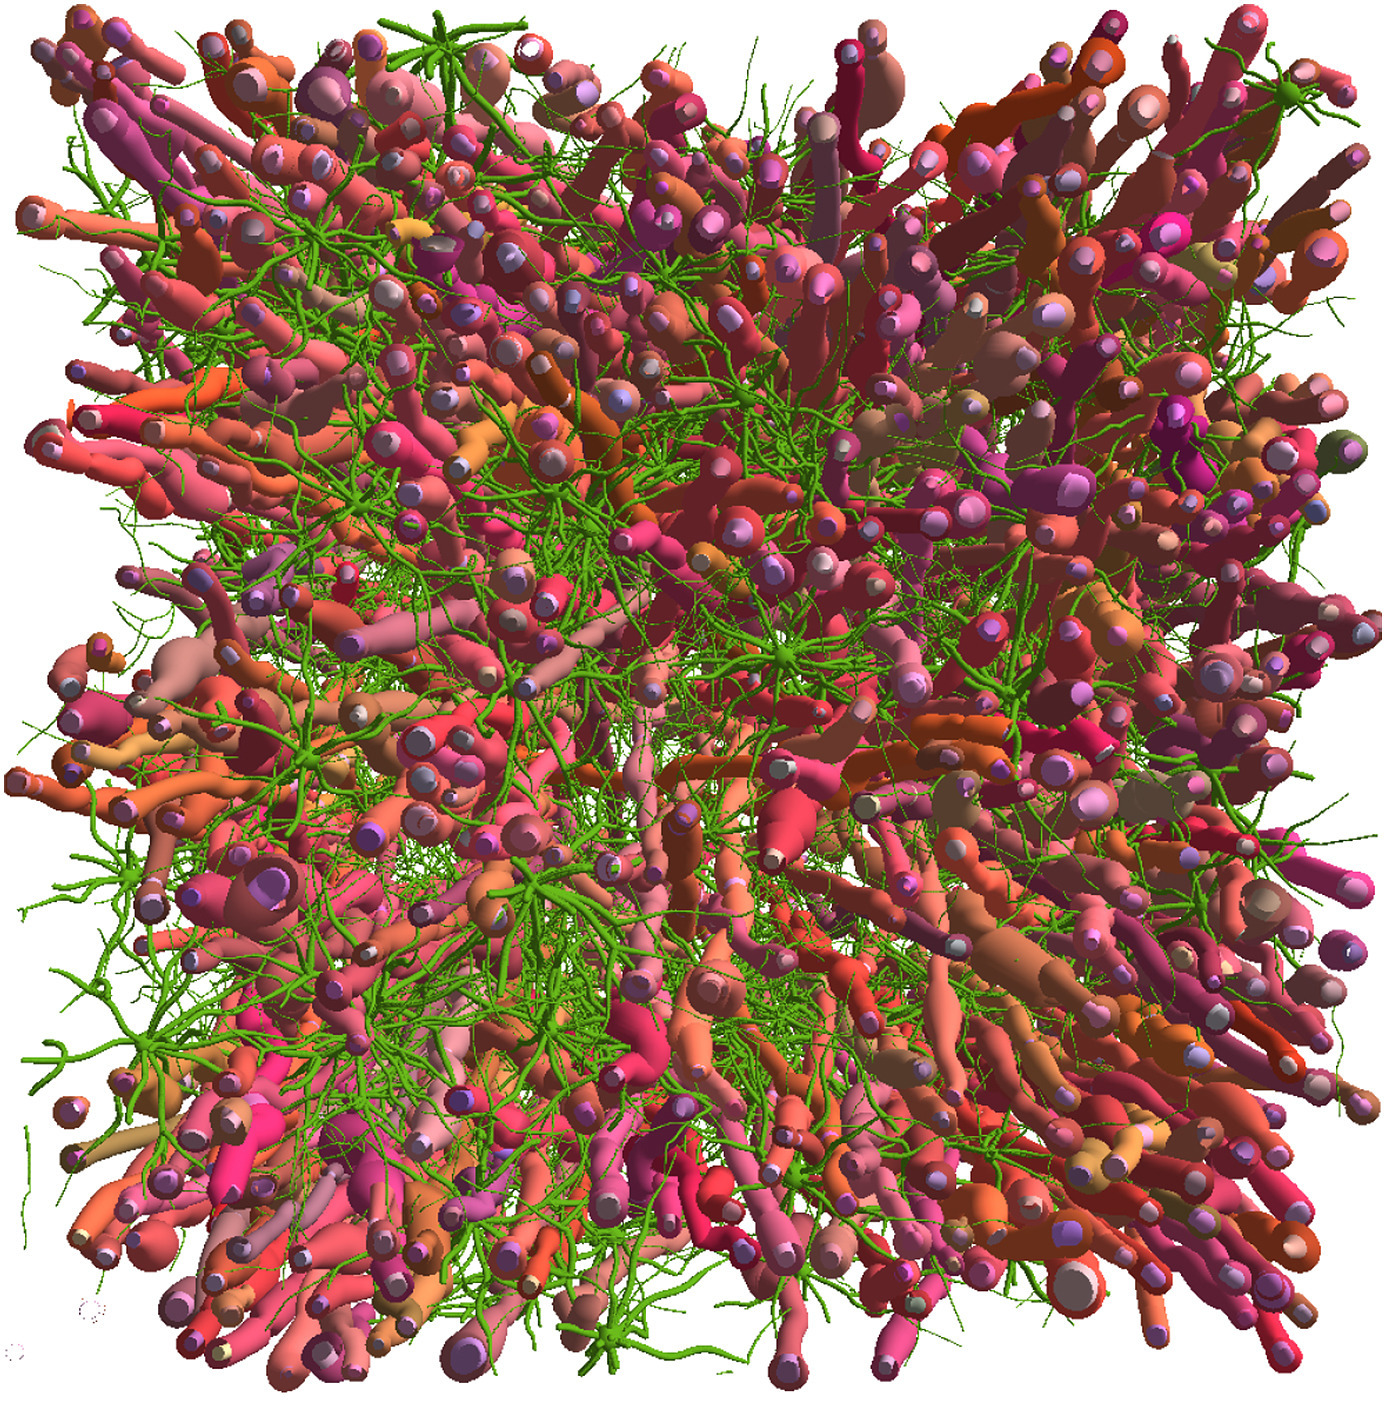
\includegraphics{gfx/model/medusa/11_.jpg}}
	\caption{11 \cite{Ginsburger2019}}
	\label{fig:medusa_11}
\end{figure}
% 
% 
% 
% 
% 
% 
% 
%
% Neurospin works with \ac{dMRI} signals.
% One focus is on the analysis of the fiber architect of the human brain.
% \ac{dMRI} is here quite handy since it is currently the only technique to allow in-vivo measurements to analyse the orientation of white matter tracts. Another importance is the availability of \ac{MRI} machines in almost every hospital in the western civilization.
% Although their resolution is with \SIrange{1.5}{3}{\tesla} limited.
% However, Neurospin is equipped with a mordern \SI{7}{\tesla} \ac{MRI}.
% This makes it possible, including higher measurments times on post mortem brain tissue, a \ac{dMRI} resolution up to \SI{200}{\micro\meter}.
% This makes it possible to allow \ac{3D-PLI} to verify and enhance the analysis of current developed tractography data. 
% %
% Along this works they developed a simulation tool (name) which is computing a Monte-Carlo simulation on the diffusion process in virtual tissues.
% Therefore, for simulations of the \ac{dMRI} signal in the brain, geometric models of nerve fibers as well as nerve cells are required.
% %
% The common goal was, due to a work packes inside the \ac{HBP}, the development of a common general purpose tool to build a geometrical library of nerve fiber configurations.
% Therefore it was decided to work based on the first approaches \cite{Ginsburger2018}.
% %
% \begin{quotation}
% We design a novel white matter numerical phantom generation algorithm which constructs biomimicking geometric configurations with few design parameters, and enables to control the level of disorder of the generated phantoms. The influence of various geometrical parameters present in white matter, such as global angular dispersion, tortuosity, presence of Ranvier nodes, beading, ...
% \end{quotation}
% %
% It is therefore qualified to generate a large database or library of parameter controlled white matter volumes.
% %
% \paragraph{differences:} 
% \begin{itemize}
%     \item All objects are aproximated with spheres.
%     \item Statistical ... of tissue
%     \item diffusion specific parameters
%     \item pathological changes like axon beeding
% \end{itemize}
